\subsubsection{UC12 - Logout}\label{UC12}

\begin{figure}[H]
  \centering
  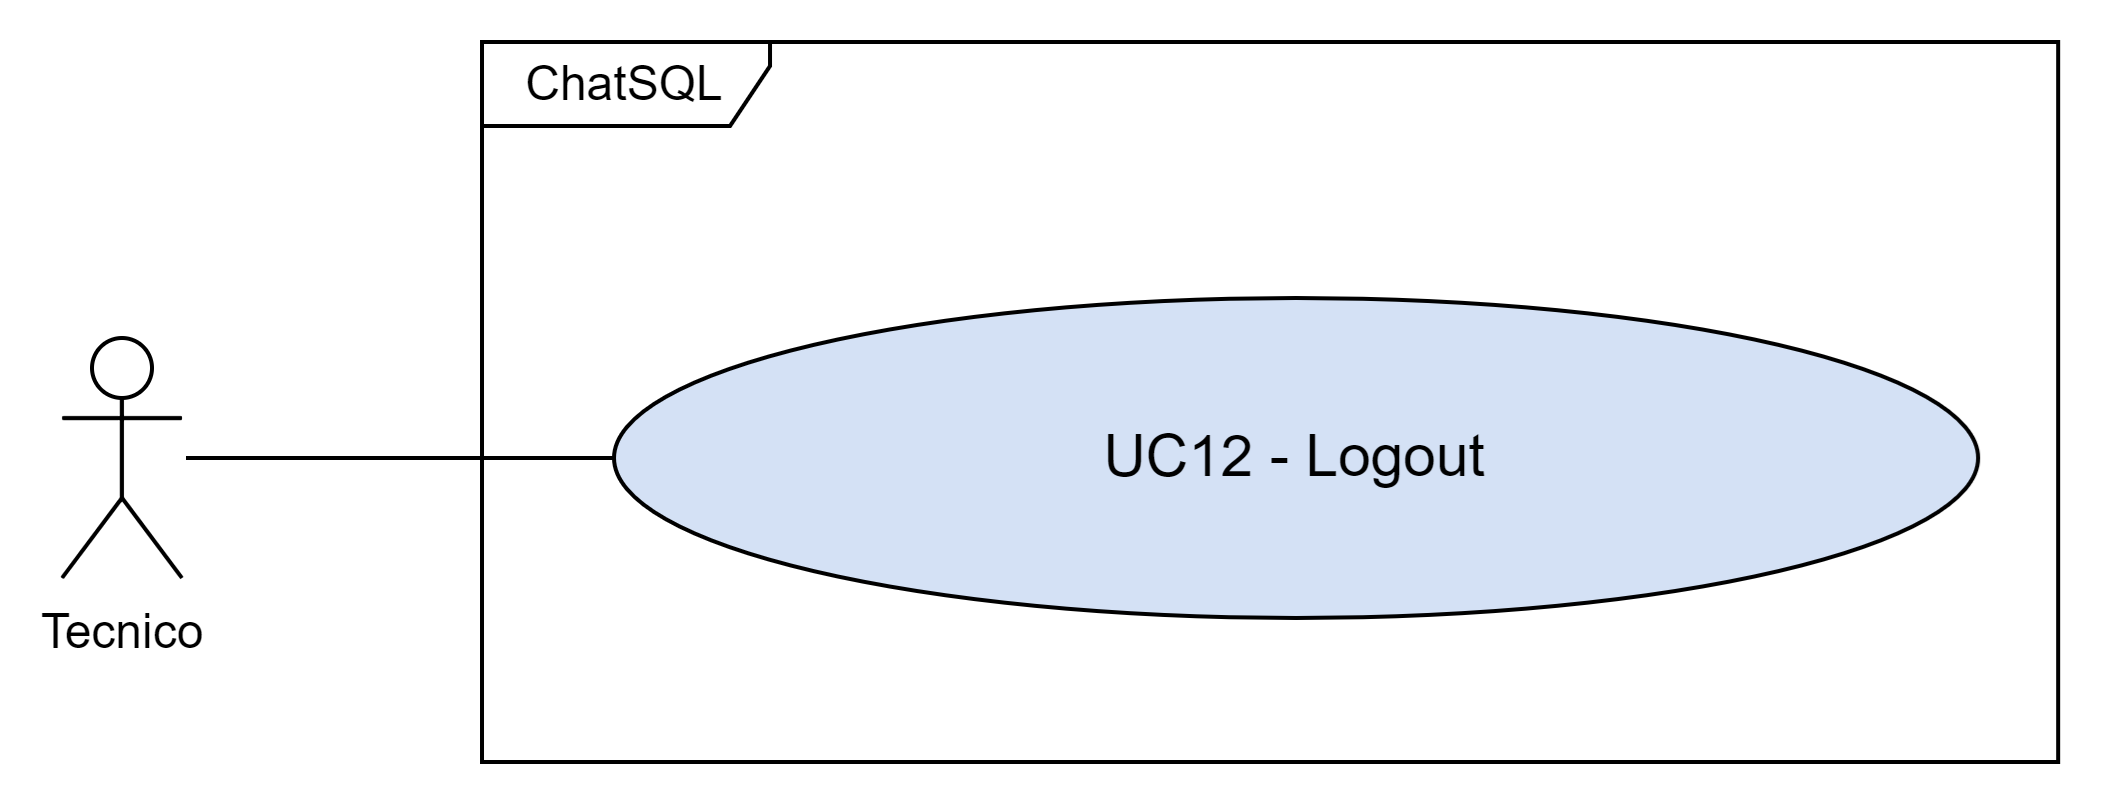
\includegraphics[width=0.90\textwidth]{assets/uc12.png}
  \caption{UC12}
\end{figure}

\paragraph*{Descrizione}
Il logout è una procedura che permette al Tecnico di disconnettersi in modo sicuro dalla piattaforma.

\paragraph*{Attori principali}
Tecnico

\paragraph*{Precondizioni}
\begin{itemize}
  \item Il Tecnico è correttamente autenticato (\hyperref[UC1]{UC1});
\end{itemize}

\paragraph*{Postcondizioni}
\begin{itemize}
  \item Il Tecnico ha eseguito il logout con successo ed ha ora a disposizione unicamente le funzionalità di un utente generico.
\end{itemize}

\paragraph*{Trigger}
L'Utente vuole effettuare il logout e terminare la sessione corrente.

\paragraph*{Scenario principale}
\begin{enumerate}
  \item Il Tecnico seleziona l'opzione "Logout";
  \item Viene avviata la procedura di logout;
  \item Il Tecnico viene disconnesso con successo dalla piattaforma;
  \item Le funzionalità proprie del Tecnico non sono più visibili.
\end{enumerate}

% Errore per il logout?
% Secondo me no
